\documentclass{standalone}
\usepackage{tikz}
\usetikzlibrary{shapes, backgrounds}
\begin{document}
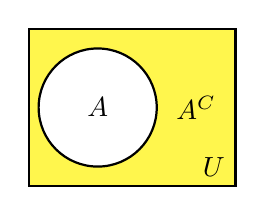
\begin{tikzpicture}[font=\sffamily]
    % Define the universe as a rectangle
    \draw[thick, fill=yellow!70] (0,0) rectangle (2.625,2);
    % Draw A
    \filldraw[fill=white, draw=black, thick] (0.875,1) circle (0.75);
    % labels
    \node[align=center] at (0.875,1) {$A$};
    \node[align=center] at (2.125,1) {$A^C$};
    \node[align=center] at (2.35,0.25) {$U$};
\end{tikzpicture}
\end{document}